%!TEX root = ../main.tex
\setcounter{chapter}{7}
\setcounter{section}{2}
\section{Design using Discrete Equivalents}
\vspace{-8pt} \hrule \hrule \hrule \hrule \hrule  \vspace{12pt}
	\begin{enumerate}
		\setcounter{enumi}{4}
		\item MMPZ
		\begin{align*}
			D_d(z) &= K_d \frac{z^{-1}}{1-e^{-5T}z^{-1}} ~~~~\mbox{where}~~ K_d \frac{1}{1-e^{-5T}} = 1 \\
			&= (1-e^{-5T}) \frac{z^{-1}}{1-e^{-5T}z^{-1}} 
		\end{align*}
		\item It is noted that Tustin and MPZ bring the similar structures each other, while ZOH and MMPZ show the similar structures, as shown in Table 8.2 
		\item Tustin and MPZ methods show a notch at $\omega_s/2$ because of their zero at $z=-1$ from $1+z^{-1}$ term. 
		\begin{figure}[h]
			\centering
			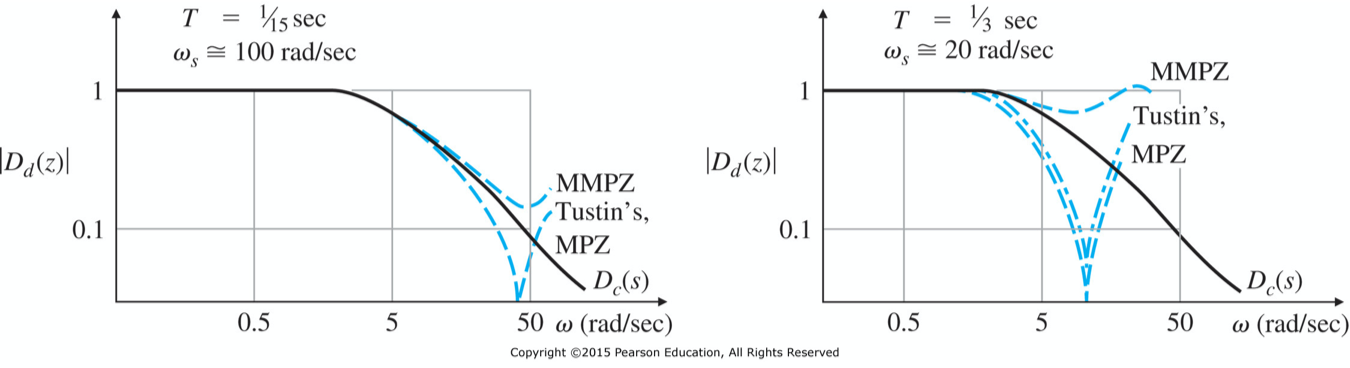
\includegraphics[width=20cm]{./FIG_Franklin/fig8-15.png}
		\end{figure}
	\end{enumerate}		